\begin{figure}
    \centering
  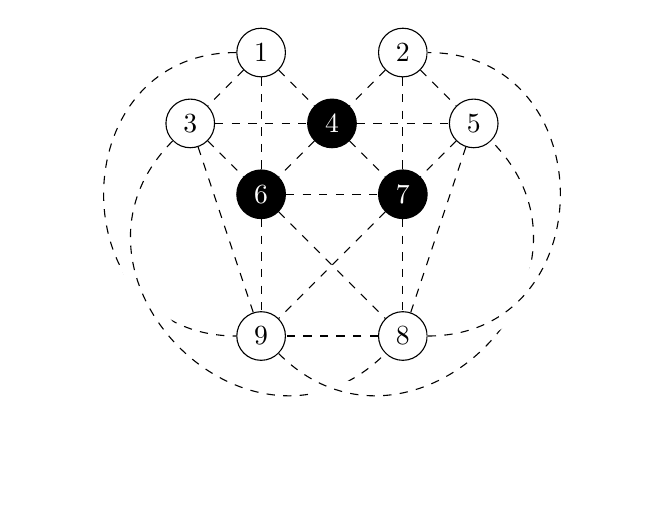
\begin{tikzpicture}[scale=0.9, rotate=0]
   \tikzstyle{nod1} = [circle, draw, fill=black, scale=1.0,
                       text = white];
   \tikzstyle{nod2} = [circle, draw, fill=white, scale=1.0];
   \tikzstyle{gd} = [black,dashed,-];

    \node[nod2] (1) at  (0,0){1};
    \node[nod2] (2) at  (2,0){2};
    
    \node[nod2] (3) at  (-1,-1){3};
    \node[nod1] (4) at  (1,-1){4};
    \node[nod2] (a5) at  (3,-1){5};
    \node[nod1] (a6) at  (0,-2){6};
    \node[nod1] (a7) at  (2,-2){7};
    \node[nod2] (a8) at (2,-4){8};
    \node[nod2] (a9) at (0,-4){9};
    
    \path[gd] (1) edge  (3);
    \path[gd] (1) edge  (4);
    \path[gd] (1) edge  (a6);
    
    \path[gd] (2) edge  (a5);
    \path[gd] (2) edge  (4);
    \path[gd] (2) edge  (a7);
    \path[gd] (3) edge  (4);
    \path[gd] (3) edge  (a6);

    \path[gd] (4) edge  (a6);
    \path[gd] (4) edge  (a7);
    \path[gd] (4) edge  (a5);
    
    \path[gd] (a5) edge  (a7);

    \path[gd] (a6) edge  (a7);
    \path[gd] (a6) edge  (a9);
    \path[gd] (a6) edge  (a8);
    
    \path[gd] (a7) edge  (a9);
    \path[gd] (a7) edge  (a8);


    %% links of a clique from another community
    % \path[thick] (4) edge  (5);
    % \path[thick] (a7) edge  (5);
    % \path[thick] (a6) edge  (5);

    \path[gd] (3) edge (a9);
    \path[gd] (a5) edge (a8);
    
    \path[gd] (1) edge 
    [bend right=90, looseness=1.6] (a9);
    
    \path[gd] (a9) edge 
    [bend right=90, looseness=1.6] (a5);

    \path[white,-] (3) edge 
    [bend right=90, looseness=1.6, line width=3mm
    ] (a8);
    \path[gd] (3) edge 
    [bend right=90, looseness=1.6] (a8);

    \path[white,-] (a9) edge 
    [bend right=90, looseness=1.6, line width=3mm
    ] (a5);
    \path[gd] (a9) edge 
    [bend right=90, looseness=1.6] (a5);

    \path[white,-] (a8) edge
    [bend right=90, looseness=1.6, line width=3mm
    ] (2);
    \path[gd] (a8) edge 
    [bend right=90, looseness=1.6] (2);

    
    \path[gd] (a8) edge  (a9);
    
  \end{tikzpicture}
    \caption{
    A $(k-1)$-clique $F$ is called {\em phantom}
    if it is contained in a (sub)graph covered by a 
    $k$-clique percolation denoted by $P$ but 
    there is no $k$-clique in $P$ that contains $F$.
    %    Alexis Baudin's definition 
    % Etant donné une percolation de 
    % k-cliques sur un graphe, une 
    % communauté est un ensemble de 
    % k-cliques.     Une **(k-1)-clique 
    % parasite** de cette communauté est une
    % (k-1)-clique qui apparait dans le 
    % graphe de la communauté mais qui 
    % n'appartient à aucune clique de la 
    % communauté.
    This figure represents a minimal example
    of a graph covered by a $k$-clique percolation
    and containing a phantom $(k-1)$-clique,
    for $k = 4$. Duplicating a node from the clique
    one can easily generate an additional
    phantom clique.
    }
    \label{gr0}
 \end{figure}

